%
% buchcover.tex -- Cover für das Buch Wavelets
%
% (c) 2018 Prof Dr Andreas Müller, Hochschule Rapperswil
%
\documentclass[11pt]{standalone}
\usepackage{tikz}
\usepackage{times}
\usepackage{geometry}
\usepackage{german}
\usepackage[utf8]{inputenc}
\usepackage[T1]{fontenc}
\usepackage{times}
\usepackage{amsmath,amscd}
\usepackage{amssymb}
\usepackage{amsfonts}
\usepackage{txfonts}
\usepackage{ifthen}
\usetikzlibrary{math}
\geometry{papersize={402mm,278mm},total={405mm,278mm},top=72.27pt, bottom=0pt, left=72.27pt, right=0pt}
\newboolean{guidelines}
\setboolean{guidelines}{true}
%\setboolean{guidelines}{false}

\begin{document}
\begin{tikzpicture}[>=latex, scale=1]
\tikzmath{
	real \ruecken, \einschlag, \gelenk, \breite, \hoehe;
	\ruecken = 2.5;
	\einschlag = 1.6;
	\gelenk = 0.7;
	\breite = 16.7;
	\hoehe = 24.6;
	real \bogengreite, \bogenhoehe;
	\bogenbreite = 2 * (\breite + \einschlag + \gelenk) + \ruecken;
	\bogenhoehe = 2 * \einschlag + \hoehe;
}

%\clip (0,0) circle (6);

\draw[fill=blue](0,0) rectangle({\bogenbreite},{\bogenhoehe});
\hsize=13.6cm

\begin{scope}
\clip (0,0) rectangle({\bogenbreite},{\bogenhoehe});
%\node at (21.2,9.0) [scale=0.145]{\includegraphics{bild.jpg}};
\node at (20.2,8.5) [scale=0.53]{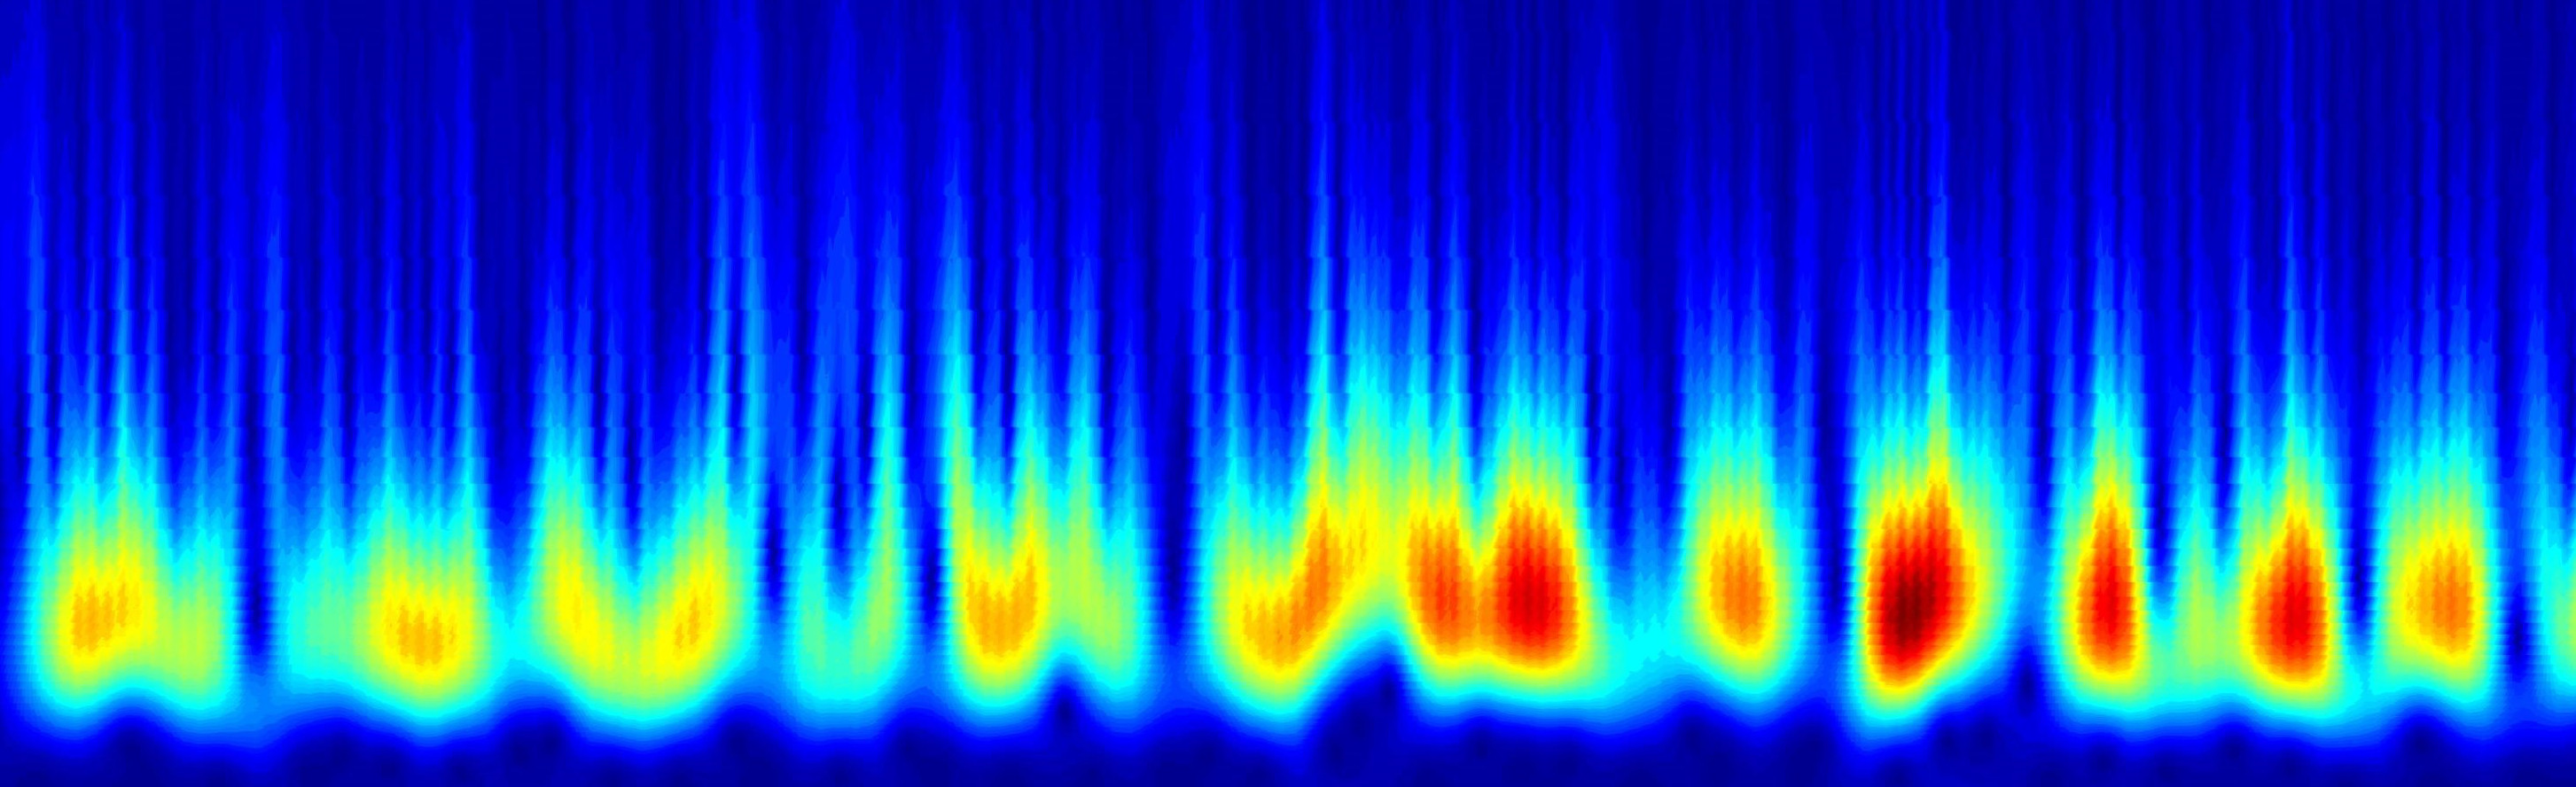
\includegraphics{gis2.jpg}};
\end{scope}

\node at ({\einschlag+2*\gelenk+\ruecken+1.5*\breite},24.3)
	[color=white,scale=1]
	{\hbox to\hsize{\hfill%
	\sf \fontsize{24}{24}\selectfont Mathematisches Seminar}};

\node at ({\einschlag+2*\gelenk+\ruecken+1.5*\breite},21.9)
	[color=white,scale=1]
	{\hbox to\hsize{\hfill%
	\sf \fontsize{50}{50}\selectfont Wavelets}};

\node at ({\einschlag+2*\gelenk+\ruecken+1.5*\breite},19.7)
	[color=white,scale=1]
	{\hbox to\hsize{\hfill%
	\sf \fontsize{13}{5}\selectfont Andreas Müller}};

\node at ({\einschlag+2*\gelenk+\ruecken+1.5*\breite},18.4)
	[color=white,scale=1]
	{\hbox to\hsize{\hfill%
	\sf \fontsize{13}{5}\selectfont
	Julian Bärtschi,
	Jonas Gründler,
	Dominic Hüppi%,
	}};

\node at ({\einschlag+2*\gelenk+\ruecken+1.5*\breite},17.75)
	[color=white,scale=1]
	{\hbox to\hsize{\hfill%
	\sf \fontsize{13}{5}\selectfont
	Raphael Nestler,
	Hansruedi Patzen,
	Cédric Renda%,
	}};

\node at ({\einschlag+2*\gelenk+\ruecken+1.5*\breite},17.1)
	[color=white,scale=1]
	{\hbox to\hsize{\hfill%
	\sf \fontsize{13}{5}\selectfont
	Michael Schmid,
	Roy Seitz,
	Manuel Tischhauser%,
	}};
 
\node at ({\einschlag+2*\gelenk+\ruecken+1.5*\breite},16.45)
	[color=white,scale=1]
	{\hbox to\hsize{\hfill%
	\sf \fontsize{13}{5}\selectfont
	Nicolas Tobler,
	Raphael Unterer,
	Kris Wyss%
	}};
 
%\node at (0,3) [color=white] {\sf \LARGE Mathematisches Seminar 2017};

% Rücken
\node at ({\bogenbreite/2 + 0.05},20.5) [color=white,rotate=-90]
	{\sf\fontsize{35}{0}\selectfont Wavelets};

% Buchrückseite
\node at ({\einschlag+0.5*\breite},18.6) [color=white] {\sf
\fontsize{13}{16}\selectfont
\vbox{%
\parindent=0pt
%\raggedright
Im Rahmen des Mathematischen Seminars der Hochschule für Technik Rapperswil
wurden im Frühjahrssemester 2019 das Thema Wavelets behandelt.
Ausgehend vom Skalarprodukt in der Vektorgeometrie wurde zunächst die
Fourier-Theorie und darauf aufbauend zunächst das einfache Haar-Wavelet
und anschliessend für technische Anwendungen besser geeignete Arten
von Wavelets studiert.
In Seminararbeiten haben die Seminarteilnehmer verschiedene Anwendungen
von Wavelets erarbeitet.
Dieses Buch bringt das Skript des Vorlesungsteils mit den von den
Seminarteilnehmern beigetragenen Seminararbeiten zusammen.

Umschlagbild: stetige Waveletanalyse mit einem komplexen Wavelet
eines Störsignals aus einer gasisolierten Schaltanlage.
}};


\ifthenelse{\boolean{guidelines}}{
\draw[white] (0,{\einschlag})--({\bogenbreite},{\einschlag});
\draw[white] (0,{\bogenhoehe-\einschlag})--({\bogenbreite},{\bogenhoehe-\einschlag});

\draw[white] ({\einschlag},0)--({\einschlag},{\bogenhoehe});
\draw[white] ({\einschlag+\breite},0)--({\einschlag+\breite},{\bogenhoehe});
\draw[white] ({\einschlag+\breite+\gelenk},0)--({\einschlag+\breite+\gelenk},{\bogenhoehe});
\draw[white] ({\bogenbreite-\einschlag-\breite-\gelenk},0)--({\bogenbreite-\einschlag-\breite-\gelenk},{\bogenhoehe});
\draw[white] ({\bogenbreite-\einschlag-\breite},0)--({\bogenbreite-\einschlag-\breite},{\bogenhoehe});
\draw[white] ({\bogenbreite-\einschlag},0)--({\bogenbreite-\einschlag},{\bogenhoehe});
}{}

\end{tikzpicture}
\end{document}
